\documentclass[12pt, a4paper]{article}
\usepackage[francais]{babel}
\usepackage[utf8]{inputenc}
\usepackage{graphicx}
\graphicspath{ {images/} }
\usepackage{color}
\usepackage{hyperref}

\title{Projet Informatique}
\author{Guo Sylvain, Rachdi Mustapha, Hoarau Romain, Paterni Thomas}
\date{Mars 2022}

\begin{document}


%************************************************************%

\maketitle
\tableofcontents
\newpage

%************************************************************%

\section{Organisation}

En choisissant de travailler dans l'environnement Visual Studio Code, nous nous sommes naturellement tournés vers une des solutions proposées par Microsoft : Live Share. Cette extension est basée sur la technologie WebRTC, ce qui permet de communiquer des données en temps réel. Cependant, cette extension ne nous permettait pas de travailler sur un même fichier à n'importe quelle heure, car il fallait qu'un membre du groupe héberge la session.

A défaut de mettre en place un serveur hébergeur, nous avons préféré nous tourner vers d'autres méthodes telles que celle proposée par Git. Nous avons choisi \emph{Github} comme hébergeur de code, puis nous avons décidé d'utiliser le logiciel \emph{Gitkraken}, qui propose une interface graphique, facilitant ainsi la compréhension. Ce logiciel nous a permis de nous concentrer sur différentes parties afin de nous répartir au mieux les tâches. La présence de l'historique nous a permis de comparer et de visualiser les différences entre plusieurs versions d'un même fichier de manière simultanée par le biais d'un écran partagé (voir \ref{fig:gitkraken}).

\begin{figure}[h] % h pour here (ci-dessous)
    \centering
    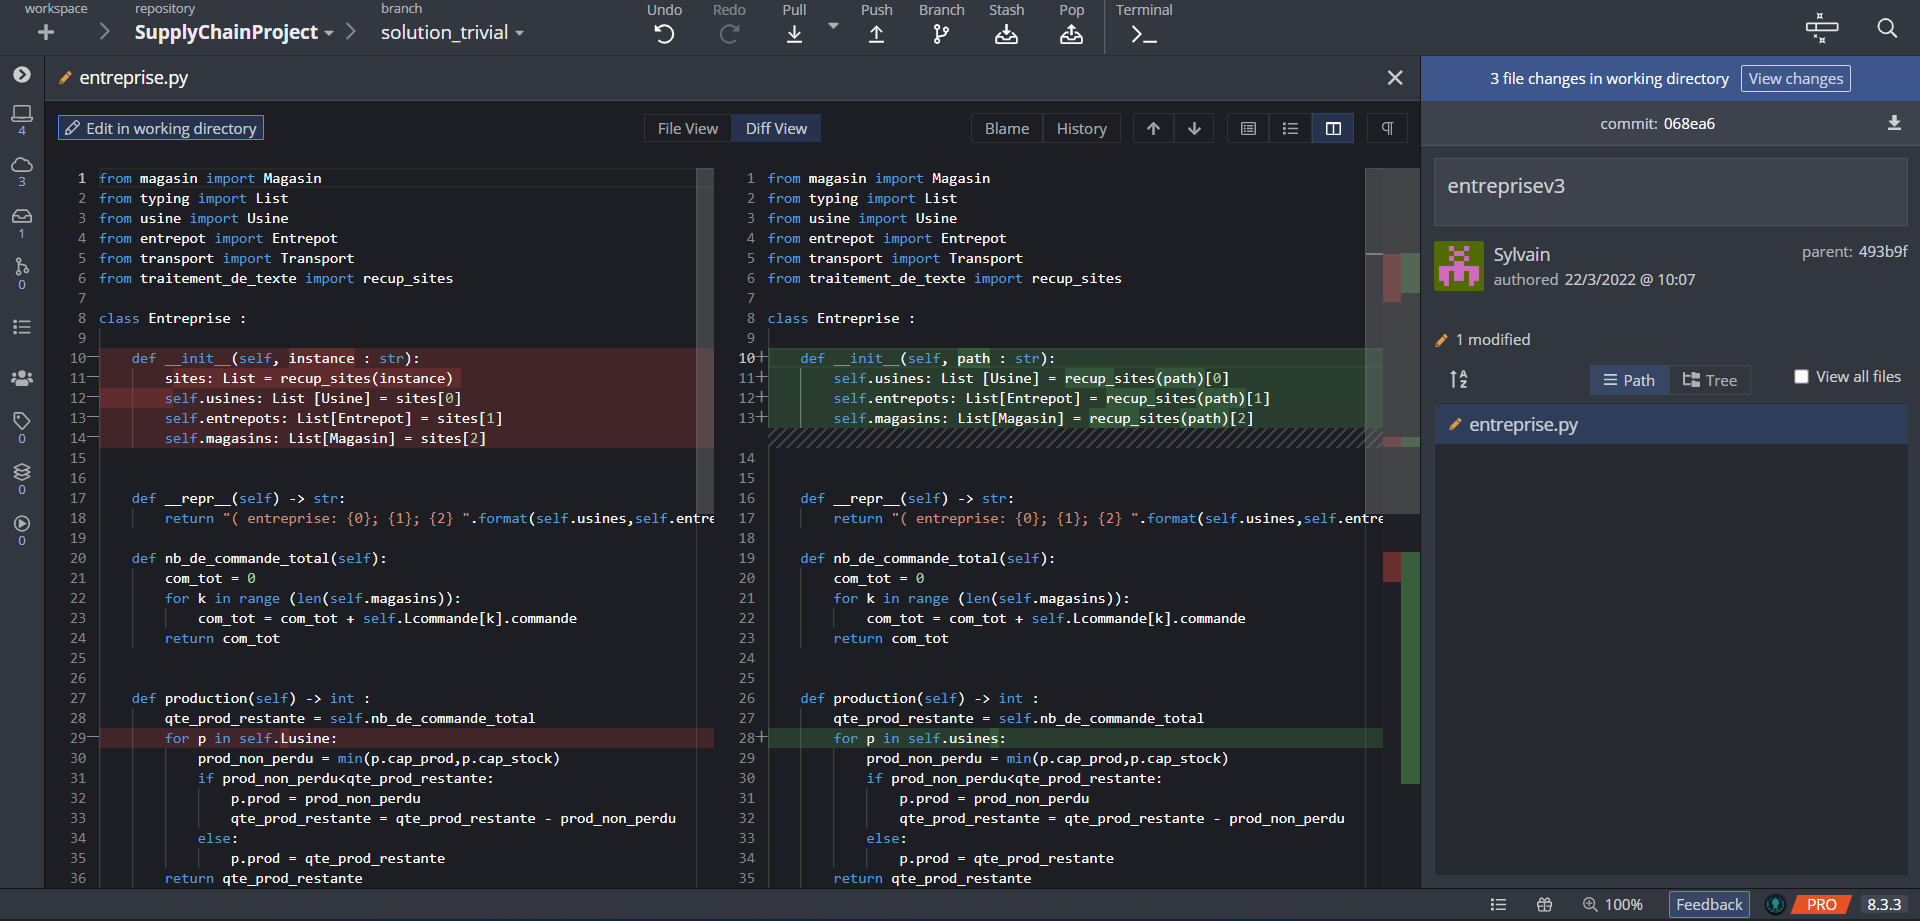
\includegraphics[width=1\textwidth]{gitkraken} % inclure l'image
    \caption{Split view de Gitkraken} % ajoute une légende
    \label{fig:gitkraken} % crée un label pour pouvoir y faire référence plus tard
\end{figure}


\noindent Le lien vers le dépôt du code est \emph{\href{https://github.com/mistertot/SupplyChainProject}{disponible ici}}.

%************************************************************%

\section{Conception logicielle}

%************************************************************%

\section{Stratégie de résolution}

%************************************************************%

\section{Bilan}


%************************************************************%
\end{document}